% !TEX root = ../sbgn_ER-level1.tex
% =============================================================================
% introduction
% =============================================================================

\chapter{Introduction}

The goal of the \textbf{S}ystems \textbf{B}iology \textbf{G}raphical \textbf{N}otation (SBGN) is to standardize the graphical/visual representation of essential biochemical and cellular processes. SBGN defines comprehensive sets of symbols with precise semantics, together with detailed syntactic rules defining their use.  It also describes the manner in which such graphical information should be interpreted. For a general description of SBGN goals, one can read:

\begin{quote}
 Nicolas Le Nov\`{e}re, Michael Hucka, Huaiyu Mi, Stuart Moodie, Falk Schreiber, Anatoly Sorokin, Emek Demir, Katja Wegner, Mirit I Aladjem, Sarala M Wimalaratne, Frank T Bergman, Ralph Gauges, Peter Ghazal, Hideya Kawaji, Lu Li, Yukiko Matsuoka, Alice Villéger, Sarah E Boyd, Laurence Calzone, Melanie Courtot, Ugur Dogrusoz, Tom C Freeman, Akira Funahashi, Samik Ghosh, Akiya Jouraku, Sohyoung Kim, Fedor Kolpakov, Augustin Luna, Sven Sahle, Esther Schmidt, Steven Watterson, Guanming Wu, Igor Goryanin, Douglas B Kell, Chris Sander, Herbert Sauro, Jacky L Snoep, Kurt Kohn, Hiroaki Kitano. The Systems Biology Graphical Notation. Nature Biotechnology 27, 735 - 741 (2009).  \url{http://dx.doi.org/10.1038/nbt.1558}
\end{quote}

This document defines the \emph{\ER{}} visual language of SBGN. \ERs are one of three views of a biological process offered by SBGN, the others being \PDs and \AFs. SBGN \ERl{} allows to see all the relationships in which a given entity participates, regardless of the temporal aspects. Entities are defined here in a broad sense as something that can exists. Relationships can be seen as rules describing the influences of entities on other relationships. An overview of \ERs is given in \sect{overview}.

% =============================================================================
% overview
% =============================================================================

To set the stage for what follows in this chapter, we first give a brief overview of some of the concepts in the \ER notation with the help of an example shown in \fig{eg1}. This example will be re-used throughout the description of the graphical symbols (glyphs) used by \SBGNERLone (with a few additions when the concepts are missing in the example) 

\begin{figure}[H]
  \centering
  \vspace*{-0.75em}
  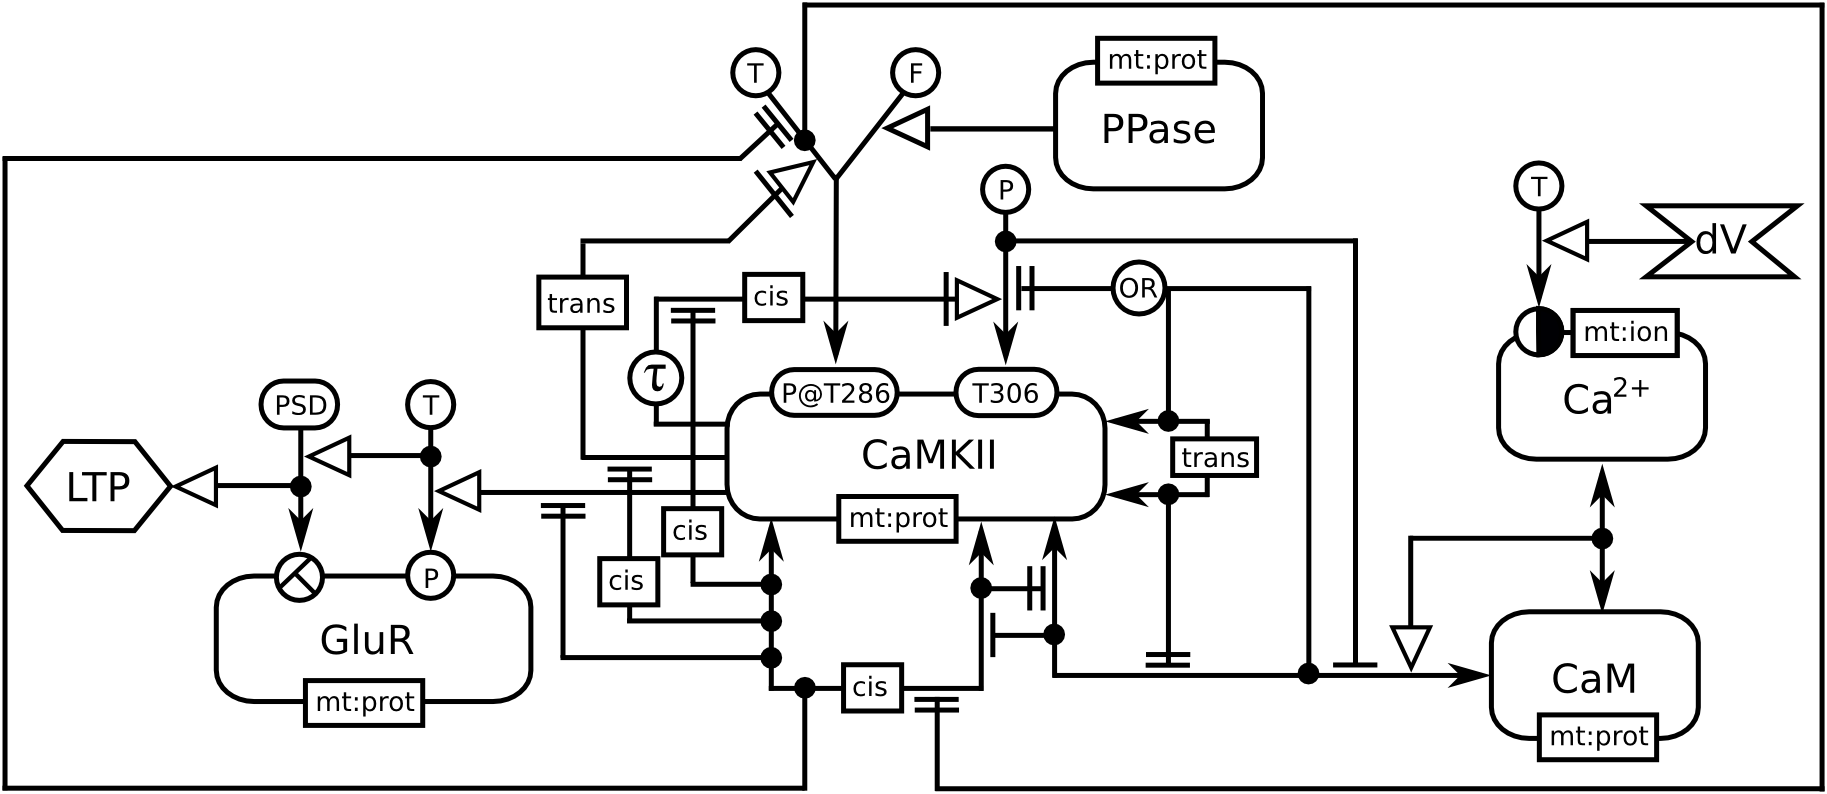
\includegraphics[scale=0.6]{examples/CaMKII-intro}
   \caption{This example of a \ER diagram depicts the effect of a depolarisation (dV) on the intracellular calcium, that binds to Calmodulin (CaM), that itself binds to the calcium/calmoduline kinase II (CaMKII). The binding of calmodulin inhibits the interaction between the catalytic and regulatory domains, thus relieving the inhibition on the kinase activity. The phosphorylation of the targets finally leads to the Long Term Potentiation (LTP) of the synapses. In addition, the diagram shows the effect of phosphorylation on threonine 286, that makes the enzyme constitutively active, and on threonine 306, that renders the kinase insensitive to calmodulin.}
  \label{fig:eg1}
\end{figure}
 
The essence of the \ER diagram is to depict the influences of entities upon the behaviour of others. The entities (in fact all interactors) are things that exist, either on their own or when statements become true. For instance, an entity can exist, different entities can interact, or a value can be assigned to an entity's property. The influences can therefore be understood as logical consequences of this existence. Contrary to the Process Diagram notation, where the different processes affect each other, the relationships are independent. On can imagine that each of the relationships represent a specific conclusion of a scientific experience or article. Their addition on a map represent the extend a the knowledge we have of the effects of the entities represented upon each other. The independence of relationships is the key to avoid the combinatorial explosion inherent to Process Diagrams.

\tab{component-summary} summarizes the different SBGN abstractions described in this chapter.
 
\newcolumntype{P}[1]{>{\raggedright\hspace{0pt}\arraybackslash}p{#1}}
 
 \begin{table}[h]
   \centering
   \small
   \begin{tabular}{@{}lP{2.4in}P{2.4in}@{}}
     \toprule
     \textbf{Component} & \textbf{Role} & \textbf{Examples}\\
     \midrule
     Interactor node
     & Something that exists
     & An entity, the result of an interaction \\[0.5em]
 
     Statement	
     & Something that can be true or false
     & An interaction between entities, the assignment of a value to a variable \\[0.5em]
 
     Influence
     & The effect of something true on the realisation of a statement or another influence.
     & A stimulation, an absolute inhibition \\
     \bottomrule
   \end{tabular}
   \caption{Summary of \ER components and their roles.}
   \label{tab:component-summary}
 \end{table}


% =============================================================================
% SBGN versioning
% =============================================================================

\section{SBGN levels and versions}
\label{sec:sbgn-levels}

It was clear at the outset of SBGN development that it would be impossible to design a perfect and complete notation right from the beginning.  Apart from the prescience this would require (which, sadly, none of the authors possess), it also would likely require a vast language that most newcomers would shun as being too complex.  Thus, the SBGN community followed an idea used in the development of other standards, i.e. stratify language development into levels.

A \emph{level} of one of the SBGN languages represents a set of features deemed to fit together cohesively, constituting a usable set of functionality that the user community agrees is sufficient for a reasonable set of tasks and goals.  Within \emph{levels}, \emph{versions} represent small evolution of a language, that may involve new glyphs, refined semantics, but no fundamental change of the way maps are to be generated and interpreted. Capabilities and features that cannot be agreed upon and are judged insufficiently critical to require inclusion in a given level, are postponed to a higher level or version.  In this way, the development of SBGN languages is envisioned to proceed in stages, with each higher levels adding richness compared to the levels below it.
% =============================================================================
% community
% =============================================================================

\section{Developments, discussions, and notifications of updates}
\label{sec:discussions}

The SBGN website (\url{http://sbgn.org/}) is a portal for all things related to SBGN.  It provides a web forum interface to the SBGN discussion list (\mailto{sbgn-discuss@caltech.edu}) and information about how anyone may subscribe to it.  The easiest and best way to get involved in SBGN discussions is to join the mailing list and participate.

Face-to-face meetings of the SBGN community are announced on the website as well as the mailing list.  Although no set schedule currently exists for workshops and other meetings, we envision holding at least one public workshop per year.  As with other similar efforts, the workshops are likely to be held as satellite workshops of larger conferences, enabling attendees to use their international travel time and money more efficiently.

Notifications of updates to the SBGN specification are also broadcast on the mailing list and announced on the SBGN website.

% =============================================================================
% typographical conventions
% =============================================================================

\section{Note on typographical convention}

The concept represented by a glyph is written using a normal font, while a \glyph{glyph} means the SBGN visual representation of the concept. For instance ``a biological entity is encoded by the SBGN ER \glyph{entity}''. 

